\chapter{基于主题的照片集故事化表达}
随着只能手机和数码摄像头的增长,人们几乎可以在任何时间任何地点拍摄照片。
大部分被拍摄的照片仅仅被存储在云端,用户很少进一步接触这部分数据,
原因在于我们缺少只能的服务去组织用户数据。因此,当前急需相关的技术和系统
将用户静态的照片总结整理成故事,使得用户能够重现社交多媒体数据中的经典时刻。
本文提出了一个基于主题的照片集故事化系统Monet,在预先定义的编辑风格上模仿
电影剪辑的手法从个人照片集中生成故事化的表达视频。该系统包含两个阶段:
照片集总结阶段从照片集中选取一部分关键照片代表整个照片集,
以及故事合成阶段用选取的照片按照主题风格生成音乐视频。在照片集总结过程中,
照片根据时间和位置信息被划分到不同的事件,再根据照片的视觉质量,所在事件的代表性,
多样性选取一部分子集作为关键性照片。第二个阶段故事合成自动根据照片的内容选取合适的
基于主题的编辑风格。每张被选取的照片通过选取合适的相机运动被转换为视频片段。然后根据
电影编辑规则将一系列的视频特效,颜色过滤器,形状和转场效果附加到视频片段中。最终的视频
和音乐混流生成故事化的音乐视频。通过实验验证,
本文提出的系统达到了比当前最好的照片集时间检测和故事合成系统更好的效果。

\section{照片集故事化表达系统框架}
从照片集中产生有吸引力和纪念意义的故事化表达面临一些挑战。首先,海量的用户照片集通常
是无序的,使得照片的浏览和分享十分枯燥。然而,照片一般来说不是随机拍摄的,而是拍摄在
不同的事件的特殊时刻。对于故事化表达来说,能够将照片组织成时间变得异常必要。
其次,由于大部分用户没有专业的拍摄技术,很多用户照片存在质量较差和内容冗余的问题。
因此,从照片集中选取一部分有代表性的子集是照片集故事化表达的关键步骤。
再次,我们需要将选取的照片用有吸引力的方式重新呈现给用户,提升用户体验。
在我们的系统中,照片集通过音乐视频的方式表达。由于照片拍摄在不同的场景,系统
需要自动选取合适的编辑风格达到的不同的表达效果。
最后,为了增加音乐视频的吸引力,
应该在视频渲染时引入视频编辑元素,如特效,形状,颜色过滤器,转场等。
从专业的视频编辑的角度,这些编辑元素依赖特定的内容和风格。因此,如何挖掘视频编辑语法,
设计基于风格的编辑元素,并将它们运用到系统中是一项具有很大挑战性但又十分必要的部分。

本文提出的基于主题的照片集故事化系统如图~\ref{fig:monet-framework}所示。用户照片首先被
组织到不同的事件中,然后在事件中选取一部分关键照片作为对照片集内容的总结。
在选取的关键照片上,系统自动为它们选取合适的编辑风格。根据预先定义的编辑语法,
系统结合相机运动,视频特效和音乐产生视频片段。最后,通过在视频片段之间添加转场效果产生
完整的音乐视频。系统实现的细节将在后续章节逐一介绍。
\begin{figure}[ht]
    \center
    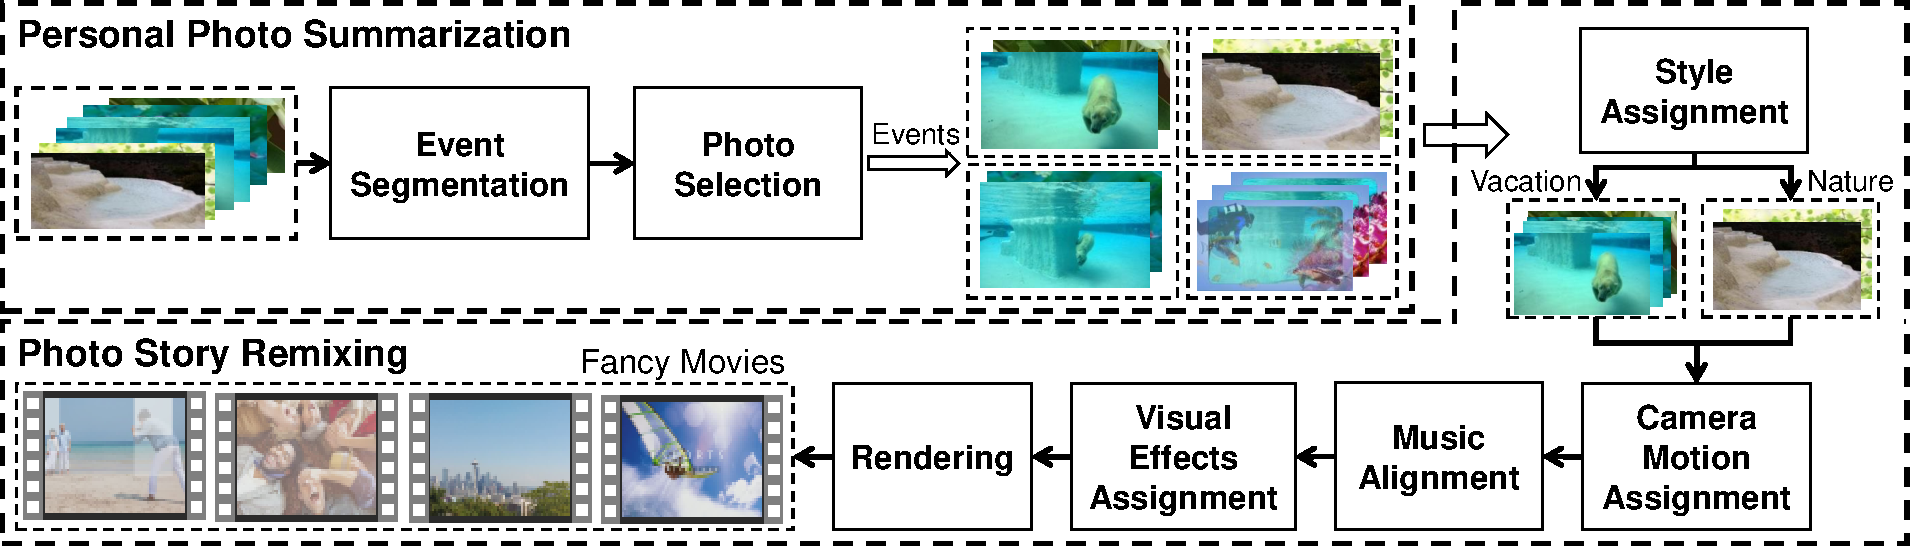
\includegraphics[clip=true, width=0.95\textwidth]{monet-framework.pdf}
    \caption{基于主题的照片集故事化表达系统框架}
    \label{fig:monet-framework}
\end{figure}

\section{照片集总结}
照片集总结包含两个步骤:事件检测和照片筛选。事件检测将照片按照事件进行组织。
照片筛选首先移除低质量或者重复的照片,然后选取高质量,有代表性,能够体现事件
均衡性的照片子集作为关键照片。

\subsection{事件检测}
从统计上来看,人们倾向于在集中的时间点拍摄照片。为了清楚地解释事件检测的概念,本文定义
``事件''如下:
\begin{definition}[\textbf{事件}]
    事件是特定的情景下、相对较短的时间段内, 用户记录值得留念的时刻的一组拍摄行为。
\end{definition}
因此,同一事件中的照片在时间和地点上比较接近。每个照片$\x_i \in \X = \{\x_1, \x_2,
\ldots, \x_N\}$属于事件$e_j \in E = \{e_1, e_2, \ldots,
e_K\}$,$N$和$K$分别是照片集$\X$中照片和事件的数目。相应地,照片$\x_i$属于事件$e_j$
的概率可以表示为$p(\x_i|e_j)$,$\x_i=(x_{i,1},
x_{i,2})$,$x_{i,1}$是时间($\mathcal{T}$),
$x_{i,2}$是GPS($\mathcal{G}$)。如果$p(e_j|x_i)$是最大的后验概率,则$x_i$被判定为
属于事件$e_j$。

给定事件$e_j$,假设时间和位置信息之间是相互独立的,似然函数$p(x_i|e_j)$被表示为:
\begin{equation}
    \label{equ:monet-priori}
    p(\x_i|e_j)= \prod_{l=1}^{2}p(x_{i,l}|e_j) = p(\mathcal{T}_i | e_j)p(\mathcal{G}_i | e_j).
\end{equation}
每个$x_{i,l}$相对于事件$e_j$的概率服从高斯分布:
\begin{equation}
    p(x_{i,l}|e_j) =
    \frac{1}{\sqrt{2\pi\delta_{j,l}^2}}e^{-\frac{(x_{i,l}-\mu_{j,l})^2}{2\delta_{j,l}^2}}.
\end{equation}
获得每个事件的分布的过程其实是学习混合高斯模型(GMM)的模型参数的过程$\Theta=\{\delta_{j,l},
\mu_{j,l}\}$。我们最大化如下目标方程所示的联合概率的对数似然函数:
\begin{equation}
    \label{equ:monet-likeli}
    l(\X;\Theta)= \log(\prod_{i=1}^N p(\x_i|\Theta)) =
    \sum_{i=1}^N \log(\sum_{j=1}^K p(e_j)p(\x_i|e_j,\Theta)),
\end{equation}
$p(x_i|e_j,\Theta)$通过方程~\eqref{equ:monet-priori}计算得到,
$p(e_j)$是事件$e_j$的先验概率。我们使用EM算法学习最优参数。在EM算法学习之前,
用K-means算法的聚类中心初始化GMM算法的模型参数。为了决定事件的数目$K$,我们在不同数值
的$K$上运用EM算法,产生一系列可能的事件分割结果。
最优的模型通过Tao等人提出的最小描述长度
(Minimum Description Length, MDL)决定~\cite{mei2006probabilistic}。

\subsection{照片筛选}
照片质量由于由于多数照片是由没有专业拍摄技巧的用户拍摄的,
我们需要滤除低质量和重复的照片,并进一步选取高质量有代表性和事件均衡性的照片子集,
从而产生高质量的故事总结。

\textbf{质量过滤}:
由于欠曝光、过曝光、模糊等问题,照片的质量可能十分低下。本文的Monet系统从$43$维
人工设计的特征评价照片质量。质量特征从以下方面提取:
\begin{itemize}
    \item 暗度(1D),亮度(1D):欠曝光和过曝光的相似比例~\cite{qa_bright};
    \item 模糊度(1D)~\cite{qa_blur},模糊差异(1D)。
        模糊差异是指照片的模糊度与高斯模糊后的模糊度之间的差值。
    \item 锐度(2D)~\cite{qa_blur,qa_sharpness},复杂性(1D)~\cite{qa_sim},
        对比度(1D)~\cite{qa_dyn_range}, 动态范围(1D)~\cite{qa_dyn_range},
        景深(1D)~\cite{qa_zhedong}。这些特征是常见的照片质量评估的全局特征(CGF)。
    \item HSV分布(12D)~\cite{qa_hsv}。照片首先会转换到HSV颜色空间,然后用
        非均匀量化将``hue''量化为8份,将``value''量化为4份。
    \item 最好块特征(7D),最差块特征(7D),主体块特征(7D)。我们发现有时候只有
        照片的一部分存在质量问题,导致整张照片被认为是是低质量照片。
        然而,全局特征并不能充分表示这种情况。因此我们提出将照片分成$5$个块(左上角,
        右上角,左下角,右下角,中间)。我们从具有最大对比度,最小对比度的块以及中间块提取
        常用的全局特征(CGF)。
\end{itemize}
我们收集了一个包含$10,361$张高质量照片和$3,134$张存在质量问题的照片的数据集,所有照片都
来自于用户拍摄的真实照片,并被人工标注为``good''或``bad''。相应地,利用上述43维特征,
我们在这个数据集上训练二分类SVM分类器。照片质量可以通过SVM模型评估,质量分数低于特定
阈值的照片将会被移除。

\textbf{重复照片过滤}:为了更好地总结照片集,我们需要检测内容重复的照片,对于
每组重复照片只保留其中一张。我们采用了Winder等人提出的局部特征将每张照片表示为$64$
维的向量~\cite{t2s2},向量的每个维度都是一个整数。照片的相似度表示为两个向量之间相同整数的个数。
如果相似度大于某个阈值,则认为它们是重复的,我们仅保留美学质量最高的照片。

\textbf{关键照片选取}:为了能够代表整个照片集的照片子集作为关键照片,我们考虑三个
因素:美学质量,代表性,事件均衡性。
\begin{itemize}
    \item \textbf{美学质量}:专业的视频制作需要选取没血质量很高的照片素材。
        我们采用了Dong等人提出的模型评价照片的美学质量~\cite{dong2014eepqa}。
    \item \textbf{代表性}:照片的代表性从两个方面进行评价:1)照片所在事件的
        重要性。当用户对某个事件更加感兴趣时,他们通常拍摄更多的照片,反之亦然。
        因此,对于事件$e_i$,如果事件中的照片数目为$n_i$,整个照片集中照片的数目为
        $N$,则事件$e_i$的重要性为$\mathcal{EI}_i=\frac{n_i}{N}$。2)多样性。
        我们需要从事件中选取多样性最大的照片子集。我们从照片中提取时间信息(
        $\t \in R^1$),位置信息($\l \in R^2$)和颜色直方图($\c\in R^{64}$)。
        照片$\x_i$和$\x_j$之间的距离定义为:
        \begin{equation}
            d_{ij} = dist(\t_i, \t_j) + dist(\l_i, \l_j) + dist(\c_i, \c_j),
        \end{equation}
        其中$dist(\a,\b)=exp(-\frac{\|\a-\b\|^2}{\sigma^2})$。

        对于照片$\x_i$,多样性定义为$\mathcal{D}_i = \sum_j d_{ij}I_{j}$。
        $I_j$是一个指示函数,当$x_j$被选为关键照片时$I_j=1$,否则$I_j=0$。
        因此,照片$x_i$的代表性为:
        \begin{equation}
            \mathcal{R}_i=\mathcal{EI}_i + \mathcal{D}_i
        \end{equation}
    \item \textbf{均衡性}:美学质量和代表性是从事件内部的粒度上选取照片,
        为了获得对照片集更加综合地总结,照片在时间上的均衡性也是一个重要的因素。
        因此,我们提出利用照片时间间隔的熵衡量均衡性。如果给定照片和前一个被选取的
        照片和下一个被选取的照片的时间间隔分别为$t_{i,i-1}$和$t_{i,i+1}$,
        照片$\x_i$的熵定义为:
        \begin{equation}
            \mathcal{E}_i=t_{i,i-1}\log t_{i,i-1} + t_{i,i+1}\log t_{i,i+1}
        \end{equation}
\end{itemize}
照片被选取的适合度是上述三个因素的线性组合:
\begin{equation}
    S_i = a \mathcal{Q}_i + b \mathcal{R}_i + c \mathcal{E}_i.
\end{equation}
其中,$a,b,c$是满足$a+b+c=1$的非负加权参数。由于代表性和均衡性依赖于整体选取的照片,
很难获取到关键照片选取的全局最优解。因此,我们用贪心算法获得关键照片子集。



\section{故事合成}
视频制作通常包括6个步骤:1)选取合适的编辑风格和背景音乐;2)基于选取的风格添加上下文
照片;3)为每个静态照片设计运动效果将其转化为运动片段;4)对每个片段运用相机运动,形状,
颜色过滤器,文本等视觉特效;5)为相邻片段选取转场效果;6)组合所有的片段和转场效果,添加
开场和结束效果产生最终的音乐视频。
一般来说,设计师需要决定编辑风格,并根据素材的语义内容设计视觉效果。

仿照上述专业视频制作的步骤,我么首先分析照片的语义内容,基于内容的语义理解,
我们为不同的照片分配不同的编辑风格,产生运动片段,并选取合适的相机运动和视觉特效和转场等效果。

\subsection{语义理解}
在视频制作过程中,素材的语义特征和内容对于风格选取,运动设计,特效制作十分重要。
在Monet系统中,我们采用了本论文提出的社交多媒体语义理解方法提取照片的语义特征。
每张照片$x_j$有$112$个可能的标签($t_i$)以及相应的概率$P(t_i|x_j)$,这些标签以及概率将会
用来判断照片属于某个风格。

为了定义编辑语法,这些标签被分成$20$个用户照片常见的类别,包括\emph{动物,建筑,暗黑,
食物,室内,室外,物体,人物,多人,人群,植物,天空,文本,山,和建筑}。此外,人脸对于
用户照片格外重要,因此我们检测人脸的数目,性别,大小和位置。照片里的人脸特征分为
``侧脸'',``一两个大比例人脸'',``一两个小比例人脸'',``三到五个小比例人脸'',``一组
小比例人脸'',``一组大比例人脸''。性别信息包括``单个人'',``单个男性'',``单个女性'',
``两个女性'',``两个男性'',``两个男性'',``夫妻'',和``人群''。所有这些特征信息将在后续
的生成视频片段,添加视觉特效等不注重使用到。

\subsection{风格选取}
本节讨论如何将照片聚类到场景以及如何为这些场景选择合适的编辑风格,
风格选取的流程如图~\ref{fig:style-assignment}所示。
\begin{figure}[ht]
    \center
    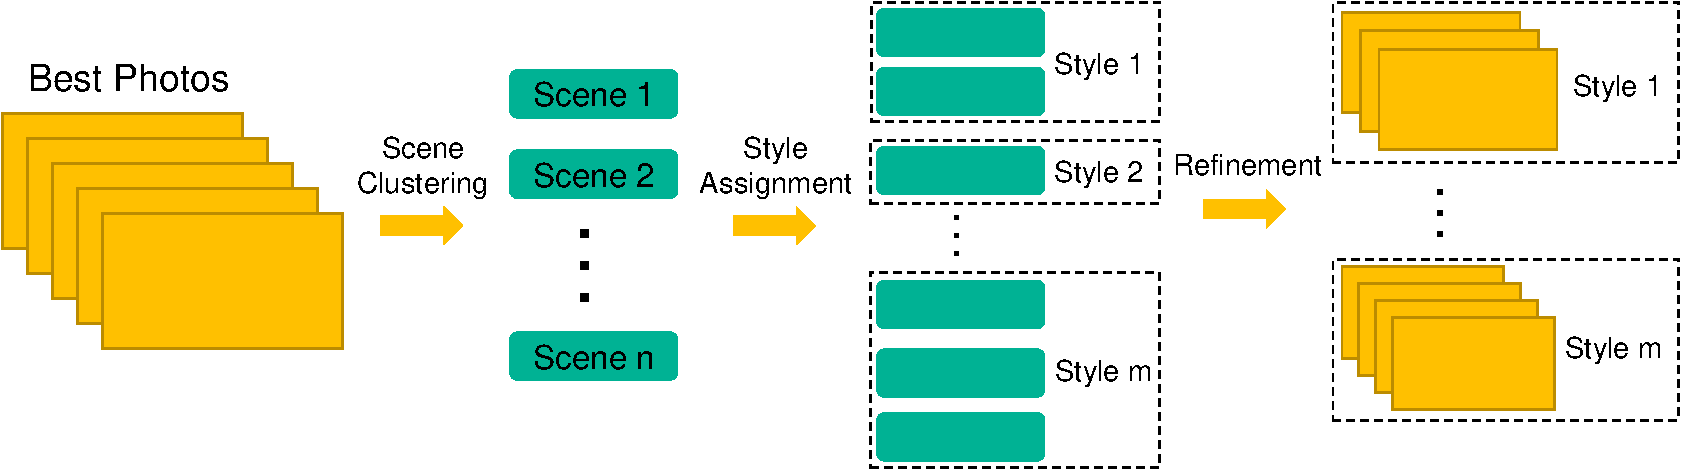
\includegraphics[clip=true, width=0.95\textwidth]{style-assignment.pdf}
    \caption{风格选取流程}
    \label{fig:style-assignment}
\end{figure}

\textbf{场景聚类}:根据我们与设计师讨论的结果,人们在特定场景中拍摄照片记录值得
纪念的时刻。换句话说,照片不仅被时间和位置信息显式地组织,同时也被场景隐式地组织。
我们的系统的主要目的是从场景中总结用户照片生成音乐视频。为了衔接照片和场景之间的联系,
每个照片用上节阐述的语义模型产生的概率向量表示$\p_i = (P(t_1|x_i), P(t_2|x_i), \ldots,
P(t_N | x_i))$。我们用Affinity Propagation(AP)~\cite{frey2007clustering}算法对照片聚类,
每个聚类中心被当做是一个场景。

\textbf{风格选取}:在我们的系统中,用不同的编辑风格表现不同的场景,使得故事化的表达
更加具有吸引力更加智能。为了决定每个场景需要使用什么编辑风格,我们用照片的语义特征训练
多类的SVM分类模型。我们邀请设计师设计了用户照片中最经常见的场景以及相关的语义词汇,如
``爱情''相关的词汇包括\emph{爱情,夫妻,甜蜜,婚礼,宝贝}。为了使得这些词汇表达的语义
是可计算的,我们用这些词从Flickr上获取至少$5,000$张照片,并用本文提出的语义理解模型将他们
提出他们的语义特征。我们训练了多类SVM分类器来区别不同的编辑风格。相应的,照片$x_k$
属于风格$\S_j$的概率表示为$P(\S_j|\p_k)$。

如果场景$scene_i$包含$M$张照片,$scene_i = \{\p_1^i, \p_2^i, \ldots,
\p_M^i\}$,该场景属于风格$\S_j$的概率为:
\begin{equation}
    P(scene_i, \mathcal{S}_j)= \sum_{k=0}^{M-1} P(\mathcal{S}_j|\textbf{p}_k^i) / M.
\end{equation}
最终,系统选取概率最大的风格编辑场景$scene_i$。
系统可能会给不同的场景选择相同的编辑风格,我们将相同风格场景的照片放到一起生成一个音乐视频。

\subsection{生成视频片段}
本文采用了Hua等人提出的照片生成视频片段的方法~\cite{hua2006photo2video},
主要包括三个步骤:
\begin{itemize}
    \item 关键帧选取。为了模拟相机运动,我们需要照片中选取全景,中景,近景作为关键帧。
    \item 生成关键帧序列。我们需要决定关键帧的播放顺序。基于电影制作的规则,我们采用了
        Hua等人提出的14种播放策略产生关键帧序列~\cite{hua2006photo2video}。
    \item 生成相机运动。最终的视频片段是通过在关键帧之间采用特定的相机运动实现的。
        对于一系列的照片,我们按照Hua等人提出的方法构建了一个合适度矩阵,通过
        最大化整体相机运动合适度和相机运动分布均衡性为每个照片选取合适的相机运动。
\end{itemize}

\subsection{音乐分析}
音乐视频需要将音乐的节奏和视频镜头的切换进行匹配。Monet系统首先对音频抽样到8kHz,
并通过Hua等人提出的方法检测音乐的节奏~\cite{hua2006photo2video}。
根据音乐的节奏和强度,系统检测最终音乐视频的切换点,从而决定生成的视频片段时长。
切换点是指音乐视频从一个视频片段切换到另一个的时间点。
切换点的检测算法将在~\ref{sec:mashup-cutpoint}中阐述,该方法提供了更好的音视频关联性,
使得视频片段的切换频率和音乐节奏更加协调。此外,该方法也尽量选择在歌唱的间歇切换,
与现有的方法在节奏点切换有明显的区别。

\subsection{故事合成}
为了生成专业的音乐视频,仅仅将视频片段和音乐混流是不够的。我们需要添加如特效,形状,
颜色过滤器,转场等视觉效果使得音乐视频更加平滑更加具有吸引力~\cite{mei2007videosense}。
为了达到这个效果,我们为每一个编辑风格设计了视觉特效模板,总结可计算的电影制作语法将
视觉效果添加到视频片段中。最终的音乐视频根据视频片段,音乐,和这些视觉特效生成。

\subsubsection{风格模板设计}
对于每个风格,我们设计了模板特效,形状,颜色过滤器和转场效果,每个视觉特效都依赖于具体
的照片内容。图~\ref{fig:monet-shape_et_example}显示了一些视觉效果的样例。
\begin{figure}[ht]
    \centering
    \subfigure[条纹效果] {
    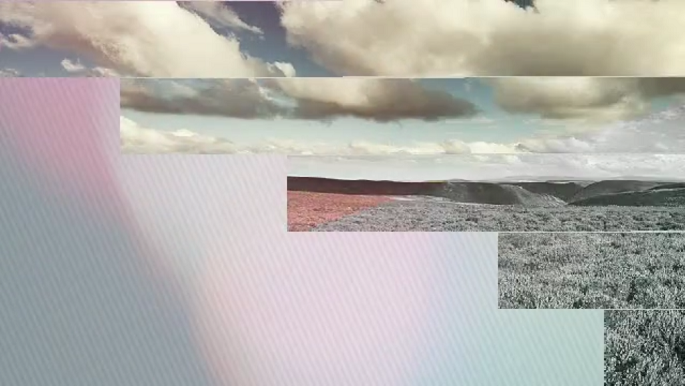
\includegraphics[width=0.23\linewidth]{multi-stripe.png}
    }
    \subfigure[叶子形状] {
    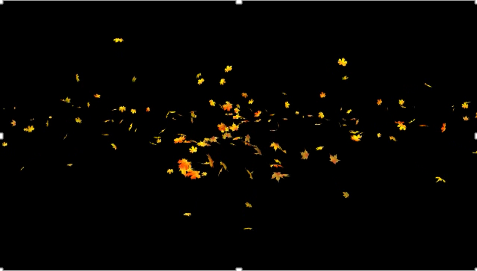
\includegraphics[width=0.23\linewidth]{shape.png}
    }
    \subfigure[阳光颜色过滤器] {
    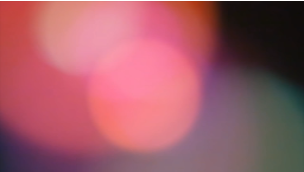
\includegraphics[width=0.23\linewidth]{color-filter.png}
    }
    \subfigure[圆形转场] {
    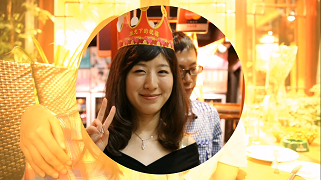
\includegraphics[width=0.23\linewidth]{transition.png}
    }
    \caption{特效,形状,颜色过滤器,转场样例。
        (a)条纹效果将照片分割成条纹依次展现,是自然主题的一种表现手法。
        (b)叶子形状中,黄色的树叶缓慢地漂浮在视频中,唤醒用户对于原始和旧时光的记忆。
        (c)将照片和阳光颜色过滤器融合能够帮助用户体验自然主题下的阳光照耀的效果。
        (d)圆形转场逐步从中间到四周展现内容,能够有效地吸引观看者的注意力到照片中的主要物体或人物。
    }
    \label{fig:monet-shape_et_example}
\end{figure}

不同的视觉效果有不同的表达效果,适用于不同的语义内容。比如,
自然风格的条纹效果(图~\ref{fig:monet-shape_et_example}(a))
适用于户外拍摄的植物或天空,但不适用于包含人的照片,因为没有用户愿意人物照片
被分割成条纹。类似的,``原始''风格中的叶子形状(图~\ref{fig:monet-shape_et_example}(b))
适用于包含草地或者树叶的照片。
``聚会''风格的圆形转场(图~\ref{fig:monet-shape_et_example}(d))特别适合照片中间仅有
一个焦点人物或物体的照片,尤其是仅包含大比例人脸的照片。甚至有效视频效果尤其是转场效果
仅适用于特定的相机运动的视频片段。总之,不同的视觉效果对于不同的语义内容和相机运动有不同的
合适度,我们为每个风格的特效、形状、颜色过滤器和转场定义了合适度语法。特效的语法规则定义
如下xml格式(形状和转场的语法类似):
\begin{itemize}
    \item \textbf{根节点$<$Grammar$>$}:根节点包含风格信息,以及特效、形状
        和转场语法的子节点。
    \item
        \textbf{特效节点$<$Effect$>$}:特效节点描述特效相对于不同语义特征和运动的合适度。
        每个特效节点包含包含一个或者多个``condition''子节点和一个可选的``percent''子节点。
        ``condition''节点包含``feature''和``score''两个子节点。如果``feature''节点以``+''
        开头,则该特效适用于该特征,如果以``-''开头,则特效不适用。``score''子节点表示特效
        适用于该特征的程度。特效节点的``percent''子节点表明该特效在所有选择特效中
        适宜出现的比例。
\end{itemize}
如果视频片段包含不适合的特征,特效的合适度则为$0$,否则特效的合适度为所有特征合适度之和。
根据视频效果语法,我们可以计算每个视频效果和每个视频片段的合适度以及部分效果期望出现的比例。


颜色过滤器的语法稍有不同。即使对于相同的视频片段,
光照和颜色分布的变化也会导致不同的表达效果。
因此,我们设计为不同的风格设计了不同的颜色过滤器,语法格式为:
\begin{itemize}
    \item \textbf{视频颜色过滤器节点$<$ColorFilter$>$}:该节点描述以视频形式出现的
        颜色过滤器的信息。``path''子节点包含视频的路径,``opacity''子节点控制过滤器视频和
        视频片段叠加时的不透明度,``overlay''子节点包含叠加的方式,``minPercent''和``maxPercent''
        控制该视频过滤器出现的最少和最大比例。
    \item
        \textbf{图片颜色过滤器节点$<$ImageFilter$>$}:该节点描述图片颜色过滤器的信息。节点内容
        与视频颜色过滤器基本相同,除了``path''子节点被替换为``name''子节点,表明预先定义的
        图片颜色过滤器。此外,图片过滤器节点包含\textbf{特效节点$<$Effect$>$}节点中的``condition''节点。
\end{itemize}
为了计算视频颜色过滤器和视频片段之间的合适度,我们首先提取颜色过滤器视频和视频片段的显著图(saliency
map)~\cite{ma2003saliency},合适度通过显著图之间的负相关系数得到。换句话说,视频颜色过滤器
不应该将用户的注意力从照片的主题内容分散到颜色过滤器上。

\subsubsection{优化视觉效果分配}
视频效果的选取可以定义为一个优化问题进行求解。
假设一共有$N_c$个视频片段,每个视频片段表示为$c_i$,一共有$N_e$个视频效果,每个表示为
$VE_j$。选取视觉效果通过确定一个选择矩阵$X=(\x_1, \x_2, \ldots,
\x_{N_C})$,$\x_j$是一个$N_e$维仅包含一个非零元素的二值向量。由于不同的视觉效果
有不同的期望出现比例(percent),我们需要首先确定它们的期望选择次数$n_j^*$。
如果$VE_j$的期望比例为$p_j$,显然$n_j^* = p_jN_c$。如果$p_j$没有指定,我们根据
它们与视频片段之间的合适度确定出现比例。假设视频片段$c_i$和视觉效果$VE_j$之间的合适度
为$S_{ij}$,$VE_j$的整体合适度为:
\begin{equation}
    S_j = \sum_{i=0}^{N_c-1}S_{ij}(1 - I_j),
\end{equation}
$I_j$是一个指示向量,当$p_j$被指定时$I_j$为1,否则为0。$VE_j$预期出现的比例为:
\begin{equation}
    p_j = \frac{S_j}{\sum_{k=0}^{N_e-1}S_{k}(1 - I_{k})}p^*,
\end{equation}
$p^* = 1 -\sum_{k=0}^{N_e-1}p_{k}I_{k}$是没有被指定比例的视觉效果能够出现在视频片段
中的剩余比例。

视频特效的选取可以归结为一个最大化整体合适度和出现比例的优化问题:
\begin{equation}
    X^* = \argmax_{X}
    \sum_{j=0}^{N_e-1}d_j\frac{\sum_{i=0}^{N_c-1}X_{ij}S_{ij}}{n_j},
\end{equation}
$d_j = exp(-\frac{(n_j-n_j^*)^2}{2})$是出现比例的分数,
用以衡量视觉效果的出现比例和预期出现比例之间的差异。

然而,仅仅只最大化合适度和出现比例可能会导致相同的相同的视觉效果被分配到
连续的视频片段。为了保持视频片段原始的顺序,保证最终视频的故事性,同时防止这种连续
效果的单一性,我们对视频效果的分布均匀性进行约束。

假设$VE_j$在$N_c$个视频片段中出现$n_j$次,我们希望$VE_j$均匀地出现在视频中。因此,
选择$VE_j$的相邻视频片段之间的预期间隔为$\frac{N_c -
n_j}{n_j}$。假设选择$VE_j$的第$k$个和第$k+1$个视频片段之间的间隔为$\delta_k$,则$VE_j$
的均匀性分数$u_{jk}$定义为:
\begin{equation}
    u_{jk} = exp(-\frac{(\delta_{k}-\frac{N_c-n_j}{n_j})^2}{2}).
\end{equation}
相应地,整体的均匀性分数为:
\begin{equation}
    U = \sum_{j=0}^{N_e-1}\frac{\sum_{k=0}^{n_j-1}u_{jk}}{n_j^*-1}.
\end{equation}

考虑到合适度,出现比例和均匀性,视频效果选取问题归结为优化如下目标方程:
\begin{eqnarray}
    X^* = \argmax_{X_{ij}}
    \sum_{j=0}^{N_e-1}(d_j\frac{\sum_{i=0}^{N_c-1}X_{ij}S_{ij}}{n_j}
    + \lambda \frac{\sum_{k=0}^{n_j-1}u_{jk}}{n_j^*-1}).
\end{eqnarray}
我们使用回溯法求解上述优化方程的最优解。

经过对用户照片集的事件检测和关键照片选取,生成视频片段,匹配音乐,以及选取视频效果以后,
Monet系统生成最终的音乐视频,对用户的照片集进行总结,并按照用户主题对用户照片集进行故事化的表达。

\section{实验结果}
据我们所知,目前还没有其他完整的系统能够自动对用户照片集进行总结并创建故事化的表达。
为了评价Monet系统的有效性,我们从照片集总结和故事合成两个角度评价Monet系统。

在实验中,所有的照片都是从用户上传的照片集中选取。为了评价照片集总结算法的效果,
我们让上传者对他们的照片进行标注,找出照片集中的事件和关键照片,并将用户照片上传到
其他事件检测和关键照片选取系统获取它们的总结结果。对于故事合成,我们邀请用户从他们的
照片集中针对每个主题风格推荐照片。然后我们随机选取一个风格并将对应的照片和音乐提交到
Monet系统和其他系统中,通过用户调查(user study)评测不同系统生成的视频。

\subsection{事件检测和关键照片选取评测}
我们邀请了6名用户分享他们在过去两年拍摄的照片,所有的照片都包含准确地拍摄时间戳,
但只有一部分包含GPS信息。用户被要求将他们的照片按照事件进行分组。对与每个事件,
他们需要为每个事件选取他们最能代表这个事件的1到6张照片作为关键照片。
这些用户标注结果被当作评测事件检测和关键照片选取的真实数据。照片集的详细情况
如表~\ref{tab:monet-photos-info}所示。
\begin{table}[htbp]
    \centering
    \caption{用户照片集详细信息} \label{tab:monet-photos-info}
    \begin{tabular}{|c|c|c|c|c|c|c|}
        \hline
        Dataset & User 1 & User 2 & User 3 &  User 4 &User 5 & User 6\\ \hline
        \#Photos & 1080 & 481 & 496 &  564 & 702 & 866 \\ \hline
        \#Events & 95 & 32 & 40 &  107 & 28 & 58 \\ \hline
        \#Best Photos & 206 & 145 & 108 &  375 & 66 & 285 \\ \hline
    \end{tabular}
\end{table}

我们采用了准确率(Precision),召回率(Recall),
和F-score来评测事件检测的效果~\cite{cooper2005temporal}。准确率表示正确检测到的
事件边界比例:
\begin{equation}
    {\text{Precision}}_{seg}=\frac{\text{\#正确检测到的事件边界}}{\text{\#检测到的事件边界}}.
\end{equation}

召回率表示正确检测到的事件边界相对真实事件边界的比例:
\begin{equation}
    {\text{Recall}}_{seg}=\frac{\text{\#正确检测到的事件边界}}{\text{\#真实事件边界}}.
\end{equation}

F-score评价综合的性能:
\begin{equation}
    \text{F-score}=\frac{2\times \text{Precision} \times \text{Recall}}{\text{Precision} + \text{Recall}}.
\end{equation}

关键照片选取通过准确率(Accuracy)评价:
\begin{equation}
    \text{Accuracy}_{best} =\frac{\text{\#正确选取的关键照片}}{\text{\#真实关键照片}}.
\end{equation}

事件检测的结果如表~\ref{tab:monet-event-seg-res}所示。可以发现,
Monet在准确率和召回率上都比PhotoToc和TEC要好,因而也
有更高的F-score。高准确率和高召回率表明Monet不仅检测到容易发现的事件边界,也能找出较难
检测的事件边界。对于关键照片选取,Monet达到了$0.68$的准确率,高于目前现有的系统(如
Google+, OneDrive, Nokia StoryTeller等)换句话说,Monet能更准确地找出能够代表照片集的关键照片。
\begin{table}[htbp]
    \centering
    \caption{事件检测结果比较}
    \label{tab:monet-event-seg-res}
    \begin{tabular}{|c|c|c|c|}
        \hline
        Method          & Precision     & Recall    & F-score \\
        \hline
        PhotoTOC\cite{platt2003phototoc} & 0.50          & 0.71      & 0.59 \\
        \hline
        TEC\cite{cooper2005temporal}      & 0.39          & 0.54      & 0.45 \\
        \hline
        Monet                    & 0.85     &   0.72    & 0.78 \\
        \hline
    \end{tabular}
\end{table}

\subsection{故事合成评测}
故事合成的客观评测比较困难,我们通过主管用户调研的评价系统性能。Monet系统一共包含10
个主题风格,我们邀请用户从他们的照片集中为每一个主题风格推荐照片。
由于不是所有用户都有所有主题风格的照片,不同的主题风格的照片可能来自不同数目的用户。
为了比较系统性能,我们为每个风格随机选取一个用户的照片作为测试数据。然后,我们将
每个风格的照片以及相应的音乐上传到Monet, Animoto, Magisto,和Tilting Slide
Show系统中,因而最终能产生总共40个音乐视频。在Animoto系统中,照片被添加特效,在背景
音乐下一次展现。Animoto为照片之间添加了转场效果,但没有考虑相机运动。在Magisto系统中,
照片伴随特效,转场,相机运动和背景音乐一起播放。在Tilting Slide Show系统中,
照片以瓷贴的形式根据音乐的节奏展现。

我们邀请了20名用户(12名男性,8名女性,用户的年龄从22岁到28岁不等)
对一共10个主题40个视频进行打分。相同风格的视频在相同页面上
按照随机顺序展现给用户。
用户从以下方面对每个视频的满意度从1到7(分数越高越好)
进行打分:

\begin{itemize}
    \item 问题1:相机运动是否合理(对比专业视频)?
    \item 问题2:视频片段之间的转场是否平滑?
    \item 问题3:整个视频的视觉效果是否有吸引力?
    \item 问题4:视频片段之间的转场是否与音乐节奏匹配?
    \item 问题5:整个视频看上去是否像专业编辑的视频?
    \item 问题6:视频是否讲述了有趣的故事?
    \item 问题7:有多少可能你愿意分享该视频给你的朋友或社交网络?
    \item 问题8:你对该视频的整体满意度是多少?
\end{itemize}

所有问题的用户打分以及平均分如表~\ref{tab:monet-story-remixing-res}所示。前4个问题是关于
故事生成的具体方面。相比于Tilting Slide Show播放静态照片和Animoto简单的相机运动,
Monet和Magisto采用了更加专业的相机运动、更丰富的特效、形状和转场,
因而它们都获得了更高的评分。Monet在相机运动和转场上的评分略低于Magisto,其中一个原因
在于Monet根据当前照片的内容选取相机运动,转场根据之前和下一个视频片段选取,视频片段
切换点也基于马尔可夫假设来确定(详见章节~\ref{sec:mashup-cutpoint}),这些方面都是基于
局部信息的。我们猜测Magisto利用了一些全局信息或者优化方法来创建更加流畅和连续的视频,
使得最终的视频编辑更具有一致性。尽管如此,Monet仍然获得了和Magisto相差无几的评分。
在视觉效果的吸引力上,Monet获得了更高的分数,
验证了本文提出的风格模板在故事合成中的有效性。

后续的四个问题是关于不同系统的整体评分。尽管Magisto在相机运动和转场上效果略好,
Monet在视频编辑的专业性上仍然获得了最高打分,再次表明Monet系统视觉效果设计和选取的
优越性。由于Magisto实现了更加平滑的转场和相机运动,它在故事性上表现更优。
尽管如此,用户在分享视频的评价上仍然更加倾向Monet系统。Monet系统在整体满意度和
平均满意度上也获得了最高的评分。这些结果表明:
1)视觉效果对于生成专业的有吸引力的视频至关重要;
2)在其他方面,Monet与当前最好的Magisto系统表现相当。
3)整体来说,Monet在照片集故事化表达上获得了最好的满意度。

\begin{table}[htbp]
    \centering
    \caption{故事生成主观评测结果}
    \label{tab:monet-story-remixing-res}
    \begin{tabular}{|c|c|c|c|c|c|c|c|c|c|}
        \hline
        & Q1 & Q2 & Q3 & Q4 & Q5 & Q6 & Q7 & Q8 & Average  \\
        \hline
        Magisto & \textbf{5.83} &\textbf{5.67} & 5.33 & \textbf{5.78} & 5.67 & \textbf{5.22} & 5.05 & 5.54 & 5.51 \\
        Animoto & 4.5 & 5 & 4.33 & 5.11 & 4.28 & 3.8 & 4.17 & 4.56 & 4.47 \\
        Monet & 5.78 & 5.60& \textbf{5.83} & 5.67 & \textbf{6} & 4.94 & \textbf{5.28} & \textbf{5.72} & \textbf{5.60} \\
        TS Show & - & 3.62 & 3.22 & 3.05 & 2.9 & 2.5 & 2.56 & 2.83 & 2.59 \\ \hline
    \end{tabular}
\end{table}

\section{小结}
本文提出了一个端到端的从用户照片集中制作基于主题的故事化表达的系统Monet。
该系统能够自动总结用户照片集并按照电影编辑语法和预先定义的编辑风格,
以有趣味性和纪念意义的音乐视频的形式叙述照片集中的故事。该系统包含两个阶段:
用户照片总结和故事合成。在照片集总结阶段,我们首先提出了一个新的多模态生成模型将用户
照片划分成事件,其次,我们根据照片的美学质量,代表性,事件的重要性从每个事件中选取一部分
关键照片代表整个照片集。在故事合成阶段,为了叙述这些关键照片,我们使用分类模型将每个照片
分配到专业编辑人员预先定义的不同编辑风格中,并将属于同一个风格的照片重新组织起来。
对于每一个照片,我们选取了特定的相机运动将它转化为动态的视频片段。为了提高最终表达
的吸引力和平滑性,我们根据视频编辑语法和视觉内容将基于风格的视觉效果运用到
视频片段中。最终,我们将视频和音乐混流生成音乐视频作为照片集的故事化表达。

本章的主要贡献包括:
\begin{itemize}
    \item 提出了自动选取照片风格的模型,
        照片的风格选取被当前故事化表达系统忽视的关键部分;
    \item 根据电影编辑语法定义了一系列编辑模板,
        使得系统可以十分高效地运用视频特效;
    \item 首次引入了多个维度的信息(音频,照片,视频)生成精美的视频表达;
    \item 系统选取关键照片的部分可以节省大量用户浏览和选取照片的时间。
        该部分也使得该系统成为首个全自动照片集故事化表达系统。
\end{itemize}

